\chapter{Bilingual RAG Museum Guide and Deployment}

\section{Overview}

The conversational guide answers a visitor's questions about an artifact---or about
the museum and ancient Egypt in general---in English or Arabic. It is a
Retrieval-Augmented Generation (RAG) system: rather than relying on a language model's
parametric memory, it retrieves relevant entries from a curated knowledge base and
passes them to the model as grounding context~\citep{lewis2020rag}. The pipeline was
developed in two iterations; this chapter describes both and explains what changed and
why.

\section{Problem and Grounding Principles}

A public museum guide must not invent history. The design therefore follows three
grounding principles: (i)~answers are constrained to retrieved museum context;
(ii)~retrieval is language-matched so an Arabic question receives Arabic context; and
(iii)~when the relevant facts are absent, the model says so rather than fabricating.
Running inference locally (no third-party LLM API) additionally removes per-request
cost and rate limits and keeps visitor queries within a controlled environment.

\section{Knowledge Base}

The knowledge base is a hand-curated set of \textbf{108 records} covering \textbf{54
unique artifacts}, each documented in both English and Arabic. A preprocessing step
fixes data-quality issues---most notably a location field that had absorbed a material
descriptor (reading ``pigment Thebes (Luxor)'' instead of ``Thebes (Luxor)'')---and
preserves the original.

Each record is split into up to three semantically distinct chunks before indexing:
an \emph{identity} chunk (name, material, location, period as discrete facts), a
\emph{description} chunk (appearance and iconography), and a \emph{significance} chunk
(historical and cultural context). The 108 records yield \textbf{215 chunks} (109
English, 106 Arabic). English and Arabic chunks are stored in \emph{separate}
collections (\texttt{\_en} and \texttt{\_ar}); a question is routed only to the
matching collection, eliminating cross-language retrieval confusion.

\section{Retrieval}

Every request begins with language detection: if more than $30\%$ of the question's
characters are Arabic script, it is treated as Arabic, otherwise English. The detected
language selects the collection and the prompt's language instruction.

In \emph{camera mode}, the app sends the English title of the detected artifact and the
retriever performs a deterministic metadata lookup, returning exactly that artifact's
chunks. In \emph{text mode}, a keyword-based query classifier assigns the question to
one of five categories and chooses a strategy accordingly (Table~\ref{tab:querycat}).
Metadata filtering guarantees \emph{completeness} for structured queries (e.g.,
``which artifacts were found at Karnak''), where similarity search would return only
the nearest chunks. A multilingual MiniLM embedding model produces comparable vectors
for English and Arabic, so the same routing serves both languages.

\begin{table}[htbp]
\centering
\caption{Text-mode query categories and retrieval strategy.}
\label{tab:querycat}
\begin{tabularx}{\textwidth}{@{}lX@{}}
\toprule
\textbf{Category} & \textbf{Retrieval strategy}\\
\midrule
Location & Metadata filter on the \texttt{was\_found\_at} field (all matching chunks).\\
Period   & Metadata filter on the historical-overview field.\\
Material & Metadata filter on the material field.\\
Royal    & Similarity search ($k=8$) against the language-matched collection.\\
Generic  & Similarity search ($k=8$) against the language-matched collection.\\
\bottomrule
\end{tabularx}
\end{table}

\section{Generation and Prompting}

The prompt has three parts: system instructions, the retrieved context, and the
question. The model is instructed to act as an Egyptology guide, to use only the
provided context, to write in flowing paragraphs without markdown (the app renders
plain text), and to give at least four sentences. For Arabic questions, the prompt adds
a reference table of the correct Arabic spellings for all fifteen royals in the dataset,
introduced after testing revealed confusions between similarly named rulers
(e.g., the Thutmose and Amenhotep kings). Generation parameters are \texttt{num\_ctx}
$=4096$, \texttt{repeat\_penalty} $=1.3$, \texttt{top\_p} $=0.9$, and
\texttt{temperature} $=0.3$; the model stays resident in GPU memory
(\texttt{keep\_alive} $=-1$). A fallback retry, triggered when a response is too short,
re-issues the prompt with an explicit instruction to answer more completely.

\section{Model Selection}

The generation model was chosen by benchmarking seven candidates against 20
standardized bilingual questions (Table~\ref{tab:funnel}). Four were eliminated:
Gemma~3n~E2B for hallucinating dimensions and locations; the default Gemma~4~E2B for
empty/truncated outputs; Qwen~3~4B because its ``thinking'' mode consumed the entire
token budget; and Qwen~3.5~4B for excessive latency and near-limit VRAM. Among the
three finalists (Table~\ref{tab:finalists}), \textbf{Gemma~4~E2B (Q4\_K\_M)} was
selected: although Llama~3.2~3B is faster, only Gemma~4~E2B~Q4 produced clean,
non-hallucinated answers in \emph{both} English and Arabic, at the lowest cold-start
VRAM.

\begin{table}[htbp]
\centering\small
\setlength{\tabcolsep}{4pt}
\caption{Candidate language models and benchmarking outcome.}
\label{tab:funnel}
\begin{tabular}{@{}lllcl@{}}
\toprule
\textbf{Model} & \textbf{Family} & \textbf{Quant.} & \textbf{VRAM} & \textbf{Verdict}\\
\midrule
Gemma 3n E2B   & Gemma & default & 1349\,MB & Eliminated (hallucination)\\
Gemma 3n E4B   & Gemma & Q3\_K\_M & 2145\,MB & Finalist\\
Gemma 4 E2B    & Gemma & default & 2021\,MB & Eliminated (empty/truncation)\\
\textbf{Gemma 4 E2B} & \textbf{Gemma} & \textbf{Q4\_K\_M} & \textbf{1389--3585\,MB} & \textbf{Selected}\\
Llama 3.2 3B   & Llama & default & 2565\,MB & Finalist\\
Qwen 3 4B      & Qwen  & default & 2907\,MB & Eliminated (thinking-mode)\\
Qwen 3.5 4B    & Qwen  & default & 3485\,MB & Eliminated (latency/VRAM)\\
\bottomrule
\end{tabular}
\end{table}

\begin{table}[htbp]
	\caption{Finalist comparison (pre-optimization).}
	\label{tab:finalists}
\begin{tabularx}{\textwidth}{@{}lXXX@{}}
	\toprule
	\textbf{Criterion} & \textbf{Gemma 3n E4B} & \textbf{Gemma 4 E2B Q4 (selected)} & \textbf{Llama 3.2 3B}\\
	\midrule
Avg.\ speed     & 19.6\,s & 22.7\,s & 7.0\,s\\
English quality & Good (minor additions) & Excellent (grounded) & Excellent (adds external facts)\\
Arabic quality  & Weak (mixed scripts) & Excellent (clean) & Unusable (garbled)\\
Hallucination   & Medium & Low & Medium\\
VRAM            & 2145\,MB & 1389\,MB (cold) & 2565\,MB\\
	\bottomrule
\end{tabularx}
\end{table}

\FloatBarrier
\section{Pipeline Optimizations}
Ten optimizations reduced end-to-end latency from over 30\,s to about 10\,s
(Table~\ref{tab:opts}, Figure~\ref{fig:latency}) while improving answer quality.

\begin{longtable}[c]{@{}>{\raggedright\arraybackslash}p{0.33\textwidth}p{\dimexpr0.67\textwidth-2\tabcolsep\relax}@{}}
	\caption{Pipeline optimizations and measured impact.\label{tab:opts}}\\
%first header
	\hline
	\textbf{Optimization} & \textbf{Measured impact}\\
	\hline
	\endfirsthead
%subsequent headers (spanning across multiple pages)
	\hline
	\textbf{Optimization} & \textbf{Measured impact}\\
	\hline
	\endhead
%subsequent footers
	\hline
	\multicolumn{2}{r}{\footnotesize(To be continued)}
	\endfoot
%end of table
	\hline
	\endlastfoot
Hierarchical chunking
(identity/description/significance)			& Replaced flat documents with semantically distinct chunks, giving the retriever precise targets. Narrow factual questions now return the identity chunk only, eliminating retrieval noise from irrelevant descriptive content.\\
%Enriched text embedding & Prepending material/location/dynasty/title into the embedded text fixed material- and location-based retrieval failures.\\
Metadata injection in prompt				& Each retrieved chunk is presented with its artifact name, material, location, and period explicitly labeled in the context block. Eliminated "I don't have that info" responses for dimension and location questions.\\
Language-separated collections
(\texttt{gem\_en}/\texttt{gem\_ar})			& Replaced the single mixed-language collection. English queries now receive only English context and Arabic queries only Arabic context, eliminating cross-language retrieval confusion.\\
Query classifier with metadata filtering	& Structured questions (location, period, material) are routed to exact field filtering instead of similarity search. An Arabic "limestone statues" query that previously returned no results now correctly returns all matching artifacts.\\
Trimmed system prompt
($\sim$500$\rightarrow$250 chars)			& $\sim$1--2\,s saved per query.\\
Mode-specific \texttt{num\_predict}
(Camera 750 / Text 900)						& $\sim$3--5\,s saved on camera-mode queries by avoiding over-generation for focused artifact questions.\\
Mode-specific \texttt{top\_k}
(Camera 4 / Text 8)							& $\sim$1--2\,s saved per camera query. Camera mode retrieves exactly the artifact's chunks; text mode retrieves enough for multi-artifact questions.\\
Flash Attention
(\texttt{OLLAMA\_\allowbreak FLASH\_\allowbreak ATTENTION=1})		& $\sim$10--15\% faster inference.\\
Composite model-instance cache key			& Fixed a silent bug where all queries used the camera token limit regardless of mode.\\
\texttt{keep\_alive}\,$=-1$					& Eliminated per-call cold-start. Model stays resident in GPU memory permanently.\\
Model pre-warming at startup				& First real request runs at warm-cache speed instead of paying the cold-start penalty.\\
\texttt{num\_ctx} raised from 1024 to 4096	& Eliminated truncated context errors for long bilingual prompts. The full system prompt and all retrieved chunks now fit within the context window.\\
\texttt{repeat\_penalty}
raised from 1.1 to 1.3						& Suppressed repeated phrases and names in responses. Previously "Thutmose III" and similar names appeared multiple times in a single sentence.\\
\texttt{top\_p} added at 0.9				& Improved Arabic token selection quality by restricting sampling to the top 90\% of the probability mass.\\
Augmented fallback retry					& Short responses are retried with an explicit instruction demanding a longer answer. Previously the retry used an identical prompt, producing the same short output.\\
Exact-location rule in system prompt		& Fixed hallucinated locations by instructing the model to use only exact location names from the context.\\
Complete Arabic royal name reference
(15 royals)									& Added all fifteen royals in the dataset to the system prompt with their correct Arabic spellings. Fixed pharaoh name confusion between similarly named rulers such as the Thutmose and Amenhotep kings.\\
\end{longtable}

\begin{figure}[htbp]
\centering
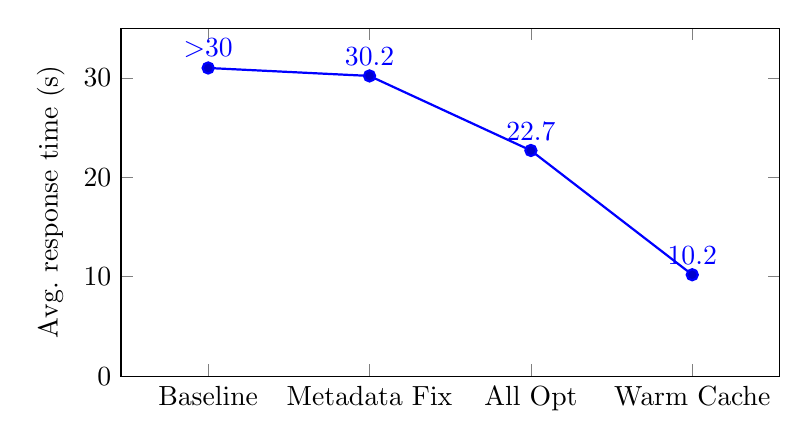
\begin{tikzpicture}
\begin{axis}[symbolic x coords={Baseline,Metadata Fix,All Opt,Warm Cache},
  xtick=data,ymin=0,ymax=35,ylabel={Avg.\ response time (s)},
  width=0.82\textwidth,height=6cm,nodes near coords,point meta=explicit symbolic,
  enlarge x limits=0.18]
\addplot+[mark=*,thick] coordinates
  {(Baseline,31)[$>$30] (Metadata Fix,30.2)[30.2] (All Opt,22.7)[22.7] (Warm Cache,10.2)[10.2]};
\end{axis}
\end{tikzpicture}
\caption{End-to-end RAG latency across optimization phases (average over the
benchmark questions): from over 30\,s to a production-ready $\sim$10.2\,s.}
\label{fig:latency}
\end{figure}

\section{From the First to the Second Iteration}

The first version loaded each record as a single flat document in one mixed-language
collection, retrieved with pure similarity search for all question types, labeled
context chunks numerically, and used a $1024$-token context window. Testing exposed
consistent weaknesses: narrow factual questions returned whole descriptions; structured
queries returned a fixed number of similar documents rather than all matches; English
questions sometimes retrieved Arabic documents; numeric context labels leaked into
answers; some Arabic names were wrong; and short responses were retried with identical
prompts. The second version addressed each as a targeted fix: dataset cleaning,
hierarchical chunking, language-separated collections, the query classifier, removal of
numeric labels, the fifteen-royal Arabic name reference, raised
\texttt{repeat\_penalty} ($1.1\rightarrow1.3$), added \texttt{top\_p} ($0.9$), a larger
context window ($1024\rightarrow4096$), and an augmented-prompt fallback.

\section{API and Deployment}

The pipeline is exposed through a FastAPI server providing \texttt{/ask},
\texttt{/ask/stream} (token streaming), \texttt{/artifact/\{id\}} (structured metadata),
and \texttt{/health}. It runs on a RunPod-hosted NVIDIA RTX A5000 instance (24\,GB
VRAM, 50\,GB RAM, 9 vCPUs) and is reached from the app over an
ngrok tunnel (Figure~\ref{fig:deploy}). At startup the server loads the ChromaDB
collections, reconstructs the indexes, and pre-warms the model so the first visitor
request is already at warm-cache speed.

\begin{figure}[htbp]
\centering
\begin{tikzpicture}[node distance=12mm and 20mm]
  \node[block] (app) {Flutter App};
  \node[block,right=of app] (api) {FastAPI (RunPod A5000)};
  \node[block,right=of api] (gemma) {Ollama\\ Gemma 4 E2B (Q4)};
  \node[store,below=of api] (chroma) {ChromaDB\\\scriptsize EN/AR};
  \draw[flow] (app) -- node[above,font=\scriptsize]{ngrok / HTTPS} (api);
  \draw[flow] (api) -- node[above,font=\scriptsize]{prompt} (gemma);
  \draw[flow] (api) -- node[right,font=\scriptsize]{retrieve} (chroma);
\end{tikzpicture}
\caption{Deployment path: the app reaches the FastAPI RAG service (on a RunPod
RTX A5000 GPU) through an ngrok tunnel; the service retrieves from ChromaDB and
prompts a local Gemma model.}
\label{fig:deploy}
\end{figure}

\section{Results}

On the full evaluation set of thirty questions spanning text mode, camera mode, and
out-of-dataset queries in both Arabic and English, the pipeline averaged about 5.9s
per answer and rated correct on all thirty responses, with no hallucinations, no truncations, 
and no retrieval misses. Performance was uniform across categories: all eight English text-mode questions, 
all six Arabic text-mode questions, all six English camera-mode questions, all three Arabic
camera-mode questions, and all three vague camera-mode questions returned complete, accurate,
well-grounded answers, while all four out-of-dataset queries (Rosetta Stone, Old Kingdom artifacts,
Great Pyramid construction, and the Rosetta Stone in Arabic) were correctly refused
without fabrication. Response times ranged from 4.33s to 8.49s, with Arabic answers
averaging roughly one second slower than English, consistent with Arabic tokenizing to 
about twice the length of equivalent English text. The evaluation also confirmed the pipeline's 
ability to synthesize across separate entries: questions about a single historical figure drew on descriptions
scattered through multiple distinct statue records to assemble a coherent biographical answer rather than
reciting a single chunk. Two cosmetic observations surfaced without affecting correctness  one English 
answer rendered a location name in its raw Arabic form, and another appended a place detail not present
in the source  both minor and isolated against an otherwise clean run.

\section{Limitations}

The knowledge base is closed: questions outside the 108 records receive limited
answers. The query classifier is keyword-based and can misroute a question that avoids
expected vocabulary. The model has no memory across requests, so follow-up questions
are answered without conversational context.

\section{Conclusion}

A fully local, bilingual RAG pipeline---ChromaDB retrieval grounding a quantized
Gemma~4~E2B model behind FastAPI---delivers factual English/Arabic museum answers at
interactive latency. The decisive gains came from grounding and targeted retrieval
fixes, not from a larger model.
